\chapter{Requisitos}

\section{Requisitos de Software}

Os requisitos de \textit{software} foram elicitados utilizando as técnicas \textit{brainstorming} e protótipo de baixa fidelidade. A partir disso, foram escritas histórias de usuário. Os critérios de aceitação e maior detalhamento das histórias serão feitos ao longo do desenvolvimento do \textit{software}.

\subsection{Protótipos}

A prototipagem é uma técnica de elicitação de requisitos que ajuda na validação de requisitos já elicitados. Através dela, o usuário pode ver as suposições do engenheiro de software e corrigi-las ou aprová-las. Também é possível elicitar novos requisitos com os protótipos existentes \cite{ieee2004swebok}.

\begin{figure}[!h]
	\centering
    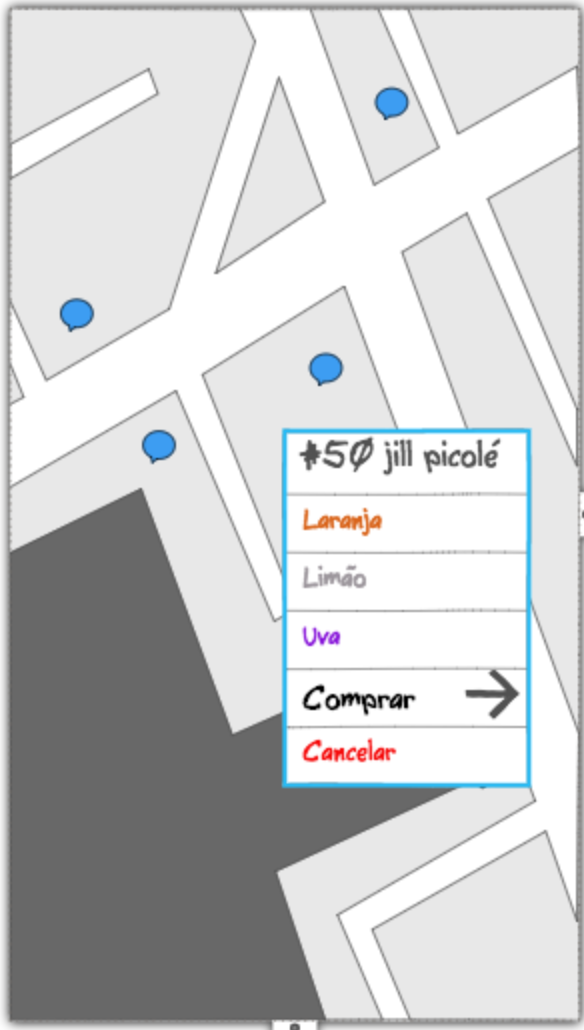
\includegraphics[scale=0.7]{figuras/home_cliente}
    \caption{Tela de seleção}
    \label{fig:home_page}
\end{figure}

\newpage

A Figura \ref{fig:home_page} representa a tela inicial do cliente. O propósito desta tela é mostrar pro cliente onde estão os sorveteiros na sua localidade. Ao selecionar um deles, aparace a lista dos sabores disponíveis naquela máquina de vendas, que pode, então ser selecionado para fazer o pedido.

Após essa seleção, o usuário vai escolher os sabores e as quantidades de sorvetes desejados, como ilustrado na Figura \ref{fig:pedido}. Esta tela apresenta os dados da máquina de vendas, como nome do vendedor e número da máquina de vendas, sabores e as formas de pagamento aceitáveis.

\begin{figure}[h]
	\centering
    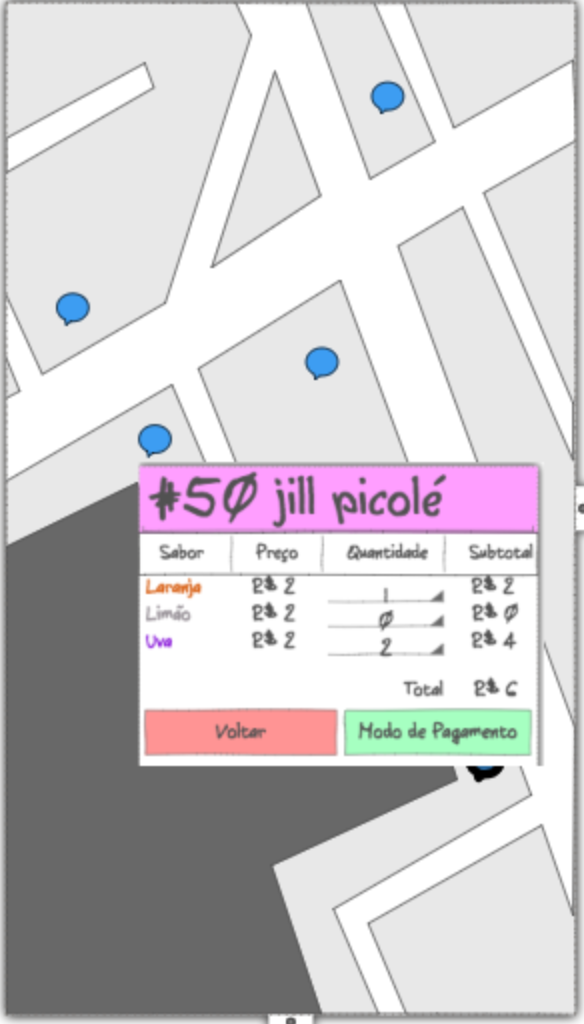
\includegraphics[scale=0.7]{figuras/pedido}
	\caption{Tela de pedido. Usuário seleciona quantidades de cada sabor desejado}
    \label{fig:pedido}
\end{figure}

\newpage

Ao escolher a forma de pagamento desejada, o usuário é redirecionado para uma página de confirmação, onde vê o resumo do seu pedido e deve entrar com os dados para realização da compra (Ver Figura \ref{fig:pagamento}). \textbf{Nenhum} dado do cartão é armazenado em nossos servidores.

\begin{figure}[h]
	\centering
    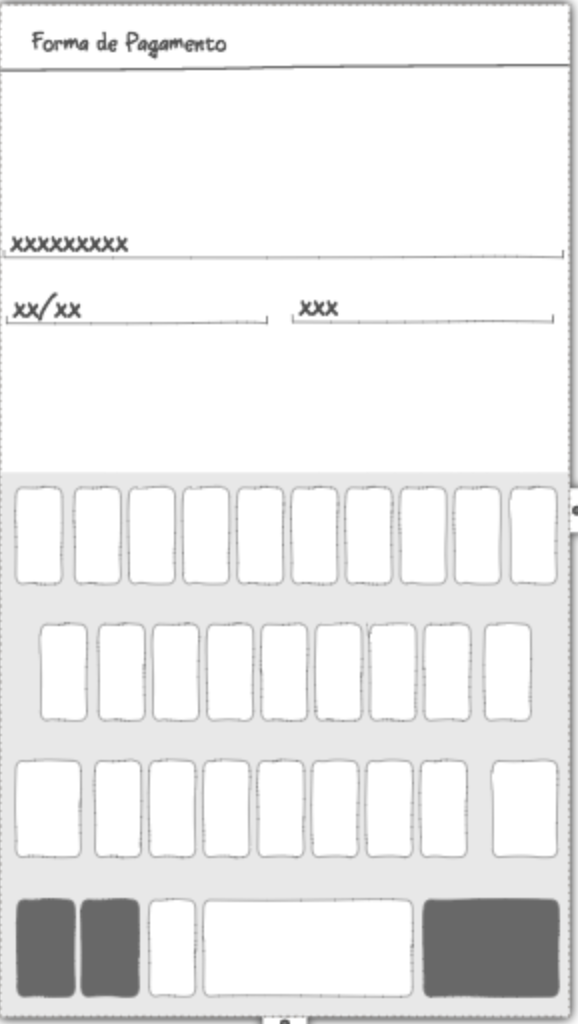
\includegraphics[scale=0.7]{figuras/pagamento}
	\caption{Tela de dados do cartão}
    \label{fig:pagamento}
\end{figure}

\newpage

Para liberar o carrinho, após o pagamento, o cliente receberia um código, que seria digitado no teclado acoplado ao carrinho. Depois de algumas discussões com os professores e o grupo, decidiu-se ter um botão no \textit{webapp}, que libera a máquina de vendas, como mostra a Figura \ref{fig:liberacao}.

\begin{figure}[H]
	\centering
    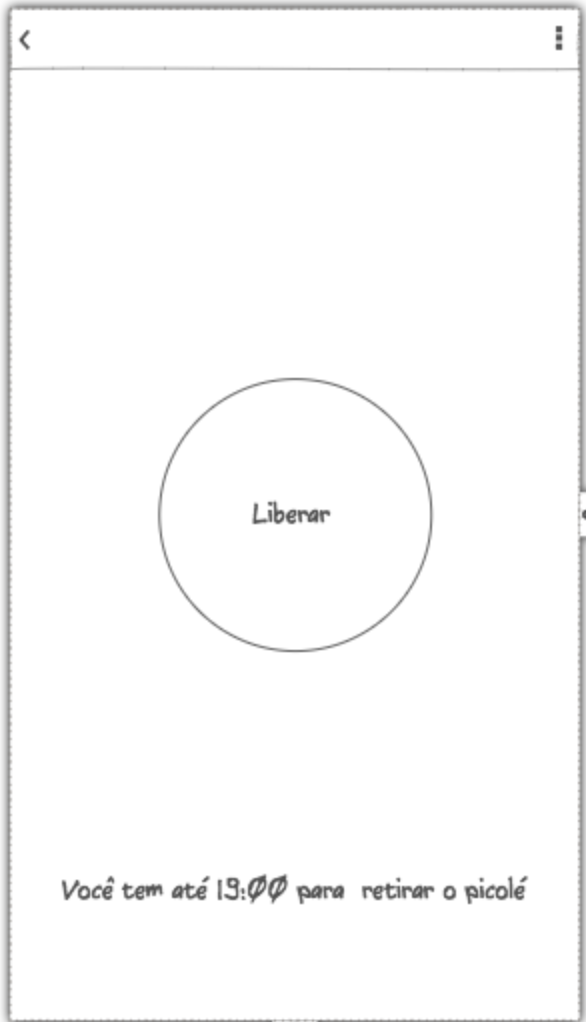
\includegraphics[scale=0.7]{figuras/liberacao}
	\caption{Liberação do picolé}
    \label{fig:liberacao}
\end{figure}

\subsection{Histórias de Usuário}
\label{sec:historias}

Uma história de usuário é uma descrição de uma funcionalidade, que pode ser válida tanto para o cliente quanto para o usuário do sistema \cite{cohn2004user}. As histórias devem ser testáveis e de curta execução, de uma a poucas semanas \cite{breitman}.

As histórias devem enfatizar a linguagem informal do usuário e não devem ser muito detalhadas até que esse detalhe seja necessário para o desenvolvimento. \cite{cohn2004advantages}

As histórias de usuário do $\pi col\acute{e}$ estão descritas abaixo.

\begin{enumerate}
\item Eu, como cliente, desejo filtrar os sabores existentes, para ver os vendedores de picolé que vendem esses sabores.
\item Eu, como cliente, desejo ver os vendedores de picolé próximos a mim para saber os quais picolés estão disponíveis.
\item Eu, como cliente, desejo ver os sabores disponíveis em cada máquina de vendas, para fazer uma escolha.
\item Eu, como cliente, desejo selecionar a quantidade dos sabores de picolés, para comprá-los.
\item Eu, como cliente, desejo selecionar uma forma de pagamento, para comprar os picolés
\item Eu, como cliente, desejo digitar meus dados de pagamento, para finalizar a compra.
\item Eu, como cliente, desejo liberar a máquina de vendas para pegar meu pedido.

\item Eu, como vendedor, desejo atualizar meu estoque, para que clientes possam comprar meu produto
\item Eu, como vendedor, desejo visualizar relatórios gerenciais para poder melhorar/analisar minhas vendas

\item Eu, como administrador, desejo visualizar relatórios de todas as minhas máquinas de venda, para poder melhorar as vendas da empresa.
\item Eu, como administrador, desejo adicionar novos sabores de picolés para diversificar meus negócios
\item Eu, como administrador, desejo modificar os preços dos picolés, para atualizá-los para o cliente.
\item Eu, como administrador, desejo adicionar vendedores à minha empresa para deixá-los fazer vendas.
\item Eu, como administrador, desejo adicionar máquinas à minha empresa para armazenar picolés.
\end{enumerate}


\section{Requisitos de Eletrônica}

Os requisitos para o sistema eletrônico da caixa de picolés são:

\begin{itemize}
	\item O amplificador de som gerar um sinal de áudio de boa qualidade sem se distorcer;
    \item O sensor de temperatura realizar a leitura correta e precisa dos dados;
    \item O sensor de presença captar um movimento perto da máquina;
    \item O módulo GPS fornecer uma localização aproximada do local;
    \item O servomotor fazer uma revolução perfeita para cada picolé vendido;
    \item O sistema de comunicação entre software e hardware.
\end{itemize}

\section{Requisitos de Estrutura}

\subsection{de Funcionamento}

\subsubsection{Mecanismo de Transporte}
\begin{itemize}
\item Acoplar e desacoplar ao freezer;
\item Garantir uma estrutura que não danifique o freezer muitos menos permita o tombamento do mesmo;
\end{itemize}

\subsubsection{Caixa de Picolés}
\begin{itemize}
\item Permitir a venda autônoma de picolés;
\item Certificar-se que a temperatura média do freezer seja -5º Celsius com margem de erro de no máximo 5º pra mais;
\item Garantir segurança à venda autônoma de picolés
\end{itemize}

\subsection{de Desempenho}
Para atingir os requisitos funcionais, a caixa de picolés deverá:
\begin{itemize}
\item Ter um sistema de refrigeração monitorado com sensor de temperatura
\item Ter uma interface de fácil entendimento para o cliente
\item Ser monitorada por um sistema de segurança com alarme
\end{itemize}

\section{Requisitos de Energia}

Com vistas à concepção e validação da solução, foram definidos os requisitos relativos ao subsistema de alimentação e refrigeração do projeto.

\begin{itemize}
\item A \textit{vending machine} deve ser capaz de manter-se resfriada por um período de aproximadamente 3 horas.
\item A placa solar deve ser capaz de carregar a bateria;
\item A máquina deve possuir uma bateria com uma capacidade suficiente para suprir o gasto energético do compressor e seus demais componentes;
\item O compressor deve ser capaz de manter o ciclo de refrigeração;
\item O inversor deve aumentar a tensão para atender às especificações do compressor;
\item O sistema de refrigeração deve ser totalmente vedado.
\end{itemize}